\section{Differential Privacy for Location Based Services}\label{sec6}
% definition of trajectory
Location Based Service (LBS) is a crucial application of mobile computing that provides personalized services based on users' geographical locations. These services, ranging from navigation assistance to location-based recommendations, require continuous collection and analysis of users' location data, often in the form of trajectories.

A trajectory is a specific type of time series that comprises spatial-temporal data. 
It can be regarded as a sequence of time-ordered points, denoted as $T=\{p_1, p_2, \cdots, p_{T}\},$ where $p_i$ represents a location and $T$ is the length of the trajectory. 
Compared with other time series, the correlations within trajectory data are more pronounced due to the constraints imposed by spatial variation. Regarding privacy levels for trajectory data, location privacy corresponds to event-level privacy, providing protection for individual locations, whereas trajectory privacy safeguards the entire trajectory.

In this section, we introduce mechanisms for handling trajectory data under differential privacy, organized according to utility improvement in location perturbation, privacy preservation against temporal correlation, and trajectory release. These mechanisms ensure that the privacy of individual locations and movements is preserved while maintaining the utility of the data for analysis and service provision.

% geo-indistinguishablility 
\subsection{Location Perturbation Based on Geo-indistinguishability}
%Geo-indistinguishability~\cite{andres2013geo} is designed to enhance utility in location perturbation. 
For meaningful outputs in LBS, the perturbed location should not deviate excessively from the actual one.   As illustrated in Fig.~\ref{geo}, constraining the perturbation domain is essential for improving utility; otherwise, a large perturbation domain yields less useful results. For example, perturbing Paris to London is impractical~\cite{andres2013geo}. Therefore, a metric-based privacy notion, $\epsilon$-geo-indistinguishability, is proposed.  Specifically, a user's level of privacy is defined as $\ell=\epsilon r$, where $r$ is the radius of the perturbation domain, corresponding to $r_i$ in Fig.~\ref{geo}. Here is the formal definition of geo-indistinguishability.
\begin{definition}[Geo-indistinguishability~\cite{andres2013geo}]
	Given any two locations $x$ and $x'$ ($d(x, x')\le r$), a randomized mechanism $M$ satisfies  $\epsilon$-geo-indistinguishability iff
	\begin{equation}\nonumber
		\mathrm{Pr}[M(x)\in Z]\le e^{\epsilon d(x, x')}\mathrm{Pr}[M(x')\in Z],
	\end{equation}
	where $Z\subseteq \mathcal{Z}$ is the possible output domain, where $d(x, x')$ represents a distance measure between $x$ and $x'$.
\end{definition}

\begin{figure}[h]
	\centering
	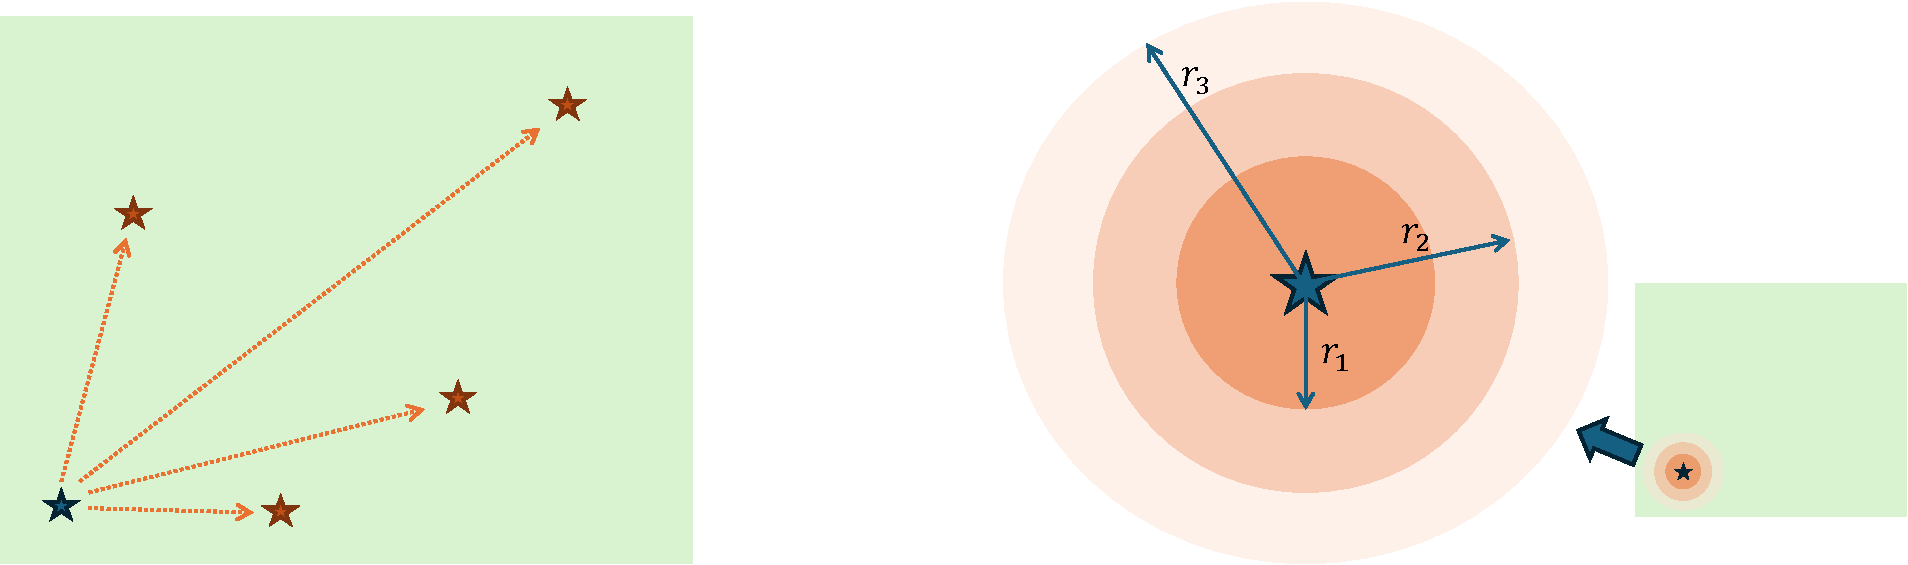
\includegraphics[width=0.8\textwidth]{submissions/submission4/figs/05-release/geo-crop.pdf}
	\caption{A traditional DP mechanism (illustrated in the left-hand figure) involves a perturbation domain (green area) for a location that is typically large, resulting in low utility for the perturbed location. To improve utility while providing useful services, a metric-based privacy notion, geo-indistinguishability, is introduced to control the perturbation (illustrated in the right-hand figure). A smaller distance $r_i$ leads to higher utility but offers less privacy. Therefore, it is important to balance the trade off between utility and privacy when designing mechanisms under geo-indistinguishability.}
	\label{geo}
\end{figure}

Since the inception of geo-indistinguishability, numerous enhancements have been made to improve the privacy notion from various perspectives.
To enhance the calculation efficiency, Bordenabe et al.~\cite{bordenabe2014optimal} proposed a method to optimize the trade-off between geo-indistinguishability and service quality in location privacy, employing linear programming to minimize service quality loss while ensuring optimal privacy guarantees. By reducing the number of constraints from cubic to quadratic, their approach significantly improves computational efficiency.
Building on the concept of geo-indistinguishability, Weggenmann and Kerschbaum~\cite{weggenmann2021differential} introduced the notion of directional privacy, a relaxation of pure differential privacy that performs effectively in the local model. 
To enhance practical utility, Zhao et al.~\cite{zhao2022geo} proposed geo-ellipse-indistinguishability to protect individual location data in directional distribution analysis. This method incorporates the covariance matrix to account for dispersion and orientation of community locations, using elliptical noise instead of circular noise. The proposed mechanisms, based on gamma and multivariate normal distributions, ensure higher probabilities of randomized locations aligning with community location trends while maintaining statistical quality.
Liang and Yi~\cite{liang2023concentrated} further advanced the concept of geo-indistinguishability by introducing concentrated geo-privacy, an update from the CDP version. This approach supports advanced composition mechanisms for high-dimensional data and achieves a lower noise scale, thereby enhancing overall privacy protection while maintaining utility. Zhao and Chen~\cite{zhao2023vector} proposed vector-indistinguishability (vector-ind) to enhance location privacy by preserving distance and direction dependencies between successive locations. They introduced four mechanisms using Laplace and Uniform distributions to achieve vector-ind, maintaining data utility while ensuring CDP.

Several mechanisms have been proposed to address various privacy issues across numerous scenarios based on geo-indistinguishability.  
Yu et al.~\cite{yu2017dynamic} proposed PIVE, a dynamic differential location privacy framework that integrates geo-indistinguishability and expected inference error to protect against inference attacks. PIVE operates in two phases: First, it identifies a protection location set based on user-defined error thresholds and prior knowledge; And then, it generates pseudo-locations within this set, ensuring differential privacy. This approach enables adaptive, personalized privacy settings tailored to individual user needs and location-based service requirements, thereby enhancing both privacy preservation and utility.
Cao et al.~\cite{cao2019priste} extended differential privacy to define $\epsilon$-spatiotemporal event privacy and proposed a framework to quantify its protection level in existing location privacy-preserving mechanisms. They demonstrated their framework by adapting the Planar Laplace Mechanism for geo-indistinguishability to ensure spatiotemporal event privacy while maintaining linear computational complexity.
Niu et al.~\cite{niu2020eclipse} introduced Eclipse, a mechanism that combines geo-indistinguishability, k-anonymity, and expected inference error to protect location privacy against long-term observation attacks. Eclipse obfuscates user locations within an anonymity set, minimizing privacy leakage while maintaining service usability and correctness.
Qiu et al.~\cite{qiu2020location}  tackled the Vehicle-based spatial crowdsourcing Location Privacy (VLP) problem, aiming to minimize travel cost distortion while preserving location privacy over road networks. They redefined geo-indistinguishability based on path distance and approximated the VLP problem as a linear programming formulation through discretization. To improve time efficiency, they proposed a two-layer optimization algorithm and analyzed the trade-off between privacy and quality of service.
Haydari et al.~\cite{haydari2022differentially} proposed a differential privacy-based map-matching algorithm (DPMM) for protecting user privacy in mobility data. DPMM generates privatized link-level location trajectories by incorporating road characteristics such as capacity and functional role. The algorithm adaptively selects the noise level based on link density, effectively balancing privacy preservation and trajectory accuracy.



% temporal correlation
\subsection{Privacy Preservation Against Temporal Correlation}
Due to the intrinsic features of location data, temporal correlations pose significant privacy issues when handling locations. Specifically, an adversary can infer information about a location based on its preceding or succeeding elements. For instance, Shao et al.~\cite{shao2020structured} proposed iTracker, a framework designed to recover multiple trajectories from differentially private data using a structured sparsity model. iTracker leverages interdependencies among locations to enhance recovery accuracy, effectively challenging existing Laplace perturbation-based location protection mechanisms.
To address privacy risks posed by temporal correlations in location data, numerous mechanisms have been proposed.
Xiao and Xiong~\cite{xiao2015protecting} introduced a solution that preserves location privacy with rigorous differential privacy guarantees by proposing $\delta$-location set, which accounts for temporal correlations in location data. They also introduced the sensitivity hull to capture geometric sensitivity in multidimensional space and presented the planar isotropic mechanism (PIM), an efficient location perturbation method that achieves optimal utility while meeting differential privacy requirements.
Cao et al.~\cite{cao2017quantifying} first investigated the privacy loss of CDP mechanisms under temporal correlations and introduced the concept of Temporal Privacy Leakage (TPL). They proposed an efficient algorithm to calculate TPL and designed methods to convert traditional DP mechanisms to ones that mitigate TPL, ensuring privacy over continuous data releases by bounding the leakage within a defined parameter $\alpha$.
Xiao et al.~\cite{xiao2017loclok} proposed LocLok, a system that protects user locations with differential privacy  by modeling temporal correlations using a hidden Markov model and applying PIM for optimal noise addition. LocLok generates possible locations via the Markov model, perturbs them with PIM, and infers true locations within a set of all possible locations, ensuring robust local privacy even when adversaries have access to historical location data.
Liu et al.~\cite{liu2019protecting} protected location privacy by analyzing the impact of temporal-spatial correlations and proposing new privacy definitions, introducing Bayesian-based geo-indistinguishability to better evaluate and enhance privacy levels. Their method optimally allocates noise among spatially and temporally correlated locations, effectively protecting sensitive locations within a trajectory while achieving differential privacy.
Ma et al.~\cite{ma2019real} proposed RPTR under $w$-event level CDP to protect real-time vehicle trajectory data. They employed dynamic sampling and ensemble Kalman filters, utilizing a position transfer probability matrix to infer correlations and ensure accurate predictions while balancing data availability and privacy. Additionally, they introduced a regional privacy weight mechanism to enhance protection in high-density areas, thereby ensuring higher prediction accuracy and adaptability across different scenarios.
Cao et al.~\cite{cao2023differentially} propose a post-processing framework to enhance the utility of differentially private streaming data releases by leveraging temporal correlations. They modeled the problem as a maximum a posterior estimation, transformed it into a nonlinear constrained programming problem, and used a transition matrix to incorporate both probabilistic and deterministic constraints.
Ahuja et al.~\cite{ahuja2023neural} proposed a method to release histogram information from trajectories under user-level CDP. To enhance utility, they introduced a method based on variational autoencoders to refine the histograms by utilizing the correlations of histograms.

\subsection{Trajectory Release Based on Perturbation or Synthesis}
 
% perturbation based release
As location-based services (LBS) become increasingly integral to everyday applications, ensuring the privacy of users while maintaining the utility of location data remains a critical challenge. Various mechanisms have been proposed to address this issue, each focusing on different aspects of location privacy and data utility. 
%A popular direction is to release trajectory data for downstream tasks. Releasing trajectory data while preserving privacy is particularly challenging due to the sensitive nature of location information.
Wang et al.~\cite{wang2022srr} introduced L-SRR, the first LDP framework for location-based services, enhancing utility while ensuring strict privacy. The proposed staircase randomized response mechanism perturbs user locations using optimized probabilities, significantly improving utility for applications such as traffic density estimation and k-nearest neighbor queries.
Cunningham~\cite{cunningham2021real} introduced a locally differentially private mechanism for trajectory data sharing that integrates public knowledge to enhance utility while ensuring privacy. This mechanism perturbs hierarchically-structured n-grams of trajectory data to capture spatio-temporal relationships, leveraging public data without compromising privacy. 
Zhang et al.~\cite{zhang2023trajectory} proposed a trajectory perturbation mechanism under user-level LDP that enhances privacy by using adjacent direction information to connect neighboring points. They introduce a two-stage pivot sampling process utilizing bi-directional clues from pivots, and an anchor-based method to restrict the spatial region of trajectories.

Synthetic trajectory generation has emerged as another promising solution, allowing for the publication of useful data without compromising individual privacy. 
Gursoy et al.~\cite{gursoy2018differentially} presented DP-Star, a framework for publishing trajectory data that ensures differential privacy while maintaining high utility. DP-Star normalizes raw trajectories using representative points, constructs a density-aware grid to preserve spatial densities, and employs a private Markov mobility model to maintain correlations and intra-trajectory mobility. This results in synthetic trajectory datasets that are both privacy-preserving and useful for various data mining tasks.
Moreover, Gursoy et al.~\cite{gursoy2018utility} presented AdaTrace, a scalable location trace synthesizer that achieves statistical privacy, deterministic attack resilience, and strong utility preservation. AdaTrace generates differentially private synthetic traces through a four-phase process: feature extraction, noise injection, and utility-aware synthesis. The synthetic traces preserve utility-critical information and are robust against Bayesian inference, partial sniffing, and outlier leakage attacks, ensuring privacy without significant utility loss.
Du et al.~\cite{du2023ldptrace} introduced LDPTrace, a locally differentially private framework for synthesizing realistic trajectories with minimal computational cost and strong privacy guarantees. LDPTrace captures key movement patterns from users' trajectories, ensuring robust statistical privacy and resilience against attacks. Extensive evaluations demonstrate that LDPTrace generates authentic trajectories without external knowledge, outperforming existing methods in terms of utility and privacy protection.
Hu et al.~\cite{hu2024real} introduced RetraSyn under $w$-event level LDP, aimed at real-time trajectory synthesis while ensuring data privacy. RetraSyn leverages mobility patterns from trajectory streams and incorporates a global mobility model, dynamic update mechanisms, and Markov-based synthesis to generate realistic trajectories. This framework effectively captures complex spatial-temporal contexts and employs adaptive privacy budget allocation strategies, ensuring authenticity and practicality in diverse real-world scenarios.
Sun et al.~\cite{sun2023synthesizing} proposed SPRT, a method for synthesizing private and realistic vehicle trajectories by incorporating geographic structures into differential privacy mechanisms. SPRT constructs a geography-aware grid to capture accurate mobility patterns and defines a moveable constraint based on real-world conditions, enhancing both summary-level statistics and individual-level mobility patterns.




